\section{Tuesday, January 30th}
\subsection{End of Unit 1: Three Inequalities}
We start by ending unit 1 with three inequalities:
\begin{enumerate}
    \item \(H[X] + H[Y] \geq H[X, Y]\)
    \begin{itemize}
        \item Interpretation: Joint entropy of independent \(X, Y\) is greater than or equal to the joint entropy of \(X, Y\).
        \item Equality requires: Independence between \(X\) and \(Y\).
        \item Proof: \(H[X] + H[Y] \geq H[X, Y] \implies H[X] + H[Y] \geq H[Y] + H[X | Y] \implies H[X | Y] \leq H[X] \implies 0 \leq H[X] - H[X | Y] \implies I(X; Y) \geq 0\), proved yesterday.
    \end{itemize}
    \item \(H[X | Y] \leq H[X]\)
    \begin{itemize}
        \item Interpretation: Observation reduces uncertainty.
        \item Equality requires: Independence between \(X\) and \(Y\).
        \item Proof: \(H[X | Y] \leq H[X] \implies 0 \leq H[X] - H[X | Y] \implies I(X; Y) \geq 0\), proved yesterday.
    \end{itemize}
    \item \(H[X | Y] + H[Y | X] \leq H[X, Y]\)
    \begin{itemize}
        \item Interpretation: Joint entropy of \(X, Y\) is greater than or equal to the expected uncertainty in one given the other.
        \item Equality requires: Independence between \(X\) and \(Y\).
        \item Proof: \(H[X | Y] + H[Y | X] \leq H[X] + H[Y | X] = H[X, Y]\), where we first use 2, then chain rule.
    \end{itemize}
\end{enumerate}

\subsection{Motivating Question: Why the log?}
To answer this, we will play a game of 20 questions:
    \begin{enumerate}
        \item What are the most efficient questions to ask?
        \item How efficient is it?
    \end{enumerate}

\subsection{Now we play a game:}
\begin{itemize}
    \item Q1: Is it alive? Yes, which we denote as \(Y_1 = 1\).
    \item Q2: Is it an animal? Yes, which we denote as \(Y_2 = 1\).
    \item Q3: Is the word 2 syllables? Yes, which we denote as \(Y_3 = 1\).
    \item Q4: Is it a Narwhal? No, which we denote as \(Y_4 = 0\).
    \item Q5: Does it live in the ocean? No, which we denote as \(Y_5 = 0\).
    \item Q6: Is it an egret? No, which we denote as \(Y_6 = 0\).
    \item (Answer: It was a rabbit).
\end{itemize}

\begin{figure}[H]
    \centering
    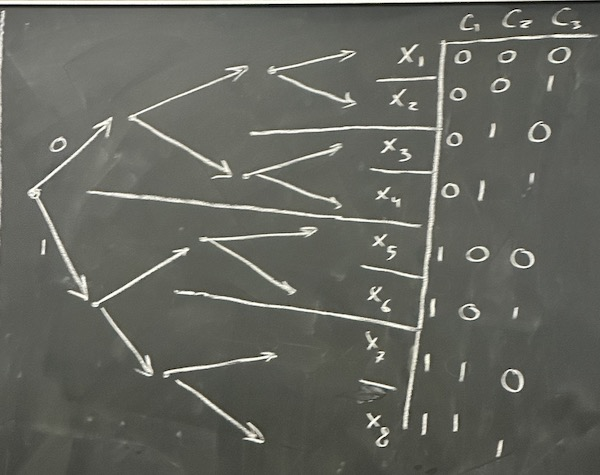
\includegraphics[scale=0.8]{lectures/wk3/img/binary_tree.jpeg}
    % \caption{Caption}
    % \label{fig:enter-label}
\end{figure}

\subsection{Motivating Question: Random Number Generation}
Given an RNG:
\begin{enumerate}
    \item How to efficiently process/transform randomness?
    \item How efficient?
\end{enumerate}


If we have \( |\mathcal{X}| = n \) outcomes, then we represent \( d^m = n \), which requires a length \( l = \lceil \log_d(n) \rceil \).

Suppose \( |\mathcal{X}| = n \), \( p \in \Delta_n \), \( p = [p_1, p_2, \ldots, p_n] \), \( p_j \geq 0 \), \( \sum_{j=1}^m p_j = 1 \), a sequence of approximations \( \{\tilde{p}^{(k)}\}^\infty \), if \( \lim_{k \to \infty} \tilde{p}^{(k)} \to p \), then, \( U(\tilde{p}^{(k)}) \to U(p) \) as \( k \to \infty \).

Restrict \( \tilde{p}^{(k)} \) to be rational, as they are dense in reals. This allows us (per the Chain Rule) to group microscopic events into macroscopic ones.

There's an equivalence between search trees and coding. In either case, you naturally get a logarithmic measure (from the depth of the tree).
